%% 
%% Copyright 2007-2020 Elsevier Ltd
%% 
%% This file is part of the 'Elsarticle Bundle'.
%% ---------------------------------------------
%% 
%% It may be distributed under the conditions of the LaTeX Project Public
%% License, either version 1.2 of this license or (at your option) any
%% later version.  The latest version of this license is in
%%    http://www.latex-project.org/lppl.txt
%% and version 1.2 or later is part of all distributions of LaTeX
%% version 1999/12/01 or later.
%% 
%% The list of all files belonging to the 'Elsarticle Bundle' is
%% given in the file `manifest.txt'.
%% 
%% Template article for Elsevier's document class `elsarticle'
%% with harvard style bibliographic references

\documentclass[preprint,12pt,authoryear]{elsarticle}

%% Use the option review to obtain double line spacing
%% \documentclass[authoryear,preprint,review,12pt]{elsarticle}

%% Use the options 1p,twocolumn; 3p; 3p,twocolumn; 5p; or 5p,twocolumn
%% for a journal layout:
%% \documentclass[final,1p,times,authoryear]{elsarticle}
%% \documentclass[final,1p,times,twocolumn,authoryear]{elsarticle}
%% \documentclass[final,3p,times,authoryear]{elsarticle}
%% \documentclass[final,3p,times,twocolumn,authoryear]{elsarticle}
%% \documentclass[final,5p,times,authoryear]{elsarticle}
%% \documentclass[final,5p,times,twocolumn,authoryear]{elsarticle}

%% For including figures, graphicx.sty has been loaded in
%% elsarticle.cls. If you prefer to use the old commands
%% please give \usepackage{epsfig}

%% The amssymb package provides various useful mathematical symbols
\usepackage{amssymb}
%% The amsthm package provides extended theorem environments
%% \usepackage{amsthm}

%% The lineno packages adds line numbers. Start line numbering with
%% \begin{linenumbers}, end it with \end{linenumbers}. Or switch it on
%% for the whole article with \linenumbers.
%% \usepackage{lineno}

\journal{Poetics}

\begin{document}

\begin{frontmatter}

%% Title, authors and addresses

%% use the tnoteref command within \title for footnotes;
%% use the tnotetext command for theassociated footnote;
%% use the fnref command within \author or \affiliation for footnotes;
%% use the fntext command for theassociated footnote;
%% use the corref command within \author for corresponding author footnotes;
%% use the cortext command for theassociated footnote;
%% use the ead command for the email address,
%% and the form \ead[url] for the home page:
%% \title{Title\tnoteref{label1}}
%% \tnotetext[label1]{}
%% \author{Name\corref{cor1}\fnref{label2}}
%% \ead{email address}
%% \ead[url]{home page}
%% \fntext[label2]{}
%% \cortext[cor1]{}
%% \affiliation{organization={},
%%            addressline={}, 
%%            city={},
%%            postcode={}, 
%%            state={},
%%            country={}}
%% \fntext[label3]{}

\title{Aligning Our Toolkits to Our Intuitions: Local Structural Models of Cultural Networks}

%% use optional labels to link authors explicitly to addresses:
%% \author[label1,label2]{}
%% \affiliation[label1]{organization={},
%%             addressline={},
%%             city={},
%%             postcode={},
%%             state={},
%%             country={}}
%%
%% \affiliation[label2]{organization={},
%%             addressline={},
%%             city={},
%%             postcode={},
%%             state={},
%%             country={}}

\author[inst1]{Omar Lizardo}

\affiliation[inst1]{organization={University of California, Los Angeles},%Department and Organization
            addressline={264 Haines Hall}, 
            city={Los Angeles},
            postcode={90095}, 
            state={CA},
            country={USA}}


\begin{abstract}
%% Text of abstract

\end{abstract}

%%Graphical abstract
%\begin{graphicalabstract}
%\includegraphics{grabs}
%\end{graphicalabstract}

%%Research highlights
\begin{highlights}
\item Research highlight 1
\item Research highlight 2
\end{highlights}

\begin{keyword}
%% keywords here, in the form: keyword \sep keyword
Cultural Networks \sep Local Structure \sep Neighborhoods \sep Exponential Random Graph Models
%% PACS codes here, in the form: \PACS code \sep code
%\PACS 0000 \sep 1111
%% MSC codes here, in the form: \MSC code \sep code
%% or \MSC[2008] code \sep code (2000 is the default)
%\MSC 0000 \sep 1111
\end{keyword}

\end{frontmatter}

%% \linenumbers

%% main text
\section{Introduction}
\label{sec:intro}
Recent years have seen a resurgence of work in cultural sociology that incorporates substantive and methodological ideas from network analysis to address core issues in studying taste, cultural consumption, and the structure and dynamics of ``cultural networks" more generally.

Despite this efflorescence of work---and perhaps very much because of it---we stand at a curious impasse in studying taste and cultural consumption. The problem is this: While the core intuitions of the field are becoming increasingly ``formalist'' and ``relationalist,''\footnote{See \citep{erikson2013formalist} for the distinction between formalist and relationism in social network analysis. The distinction is undoubtedly important but not crucial for my broad argument. Therefore, in what follows, I will use ``formalist,'' ``formalism'', ``relational,'' and ``relationalist'' interchangeably to refer to the cluster of intuitions that come packaged with network analytic thinking and which have been increasingly used to understand cultural tastes} the core workhorse methods in the field, such as traditional regression analysis (and its various non-linear and mixed effects variations), latent class analysis, various data reduction techniques like factor and cluster analysis, and the now widely used geometric data analytic techniques only cash in those formalist intuitions in either very indirect or roundabout ways. 

Meanwhile, the suite of network-inspired techniques that have been recently introduced, while useful for recasting core notions in a more relational mold, lack the natural unity and compatibility with thinking of the world as governed by chance, uncertainty, and probability as statistically grounded techniques like the general linear model or latent class analysis. 

In this paper, I argue that a general, statistically and probabilistically grounded approach to thinking about how the local structuration of network ties gives rise to macro-structural patterns tied to a now relatively accessible, well-developed and mature framework for the statistical analysis of network structures---typically going by the offputting and unwieldy name of ``exponential random graph models,'' can serve to align the increasingly formalist intuitions quantitatively inspired cultural analysis bring to the study of tastes and culture consumption, with a coherent methodological approach that cashes in those intuitions \textit{directly}, while at the same time incorporating into a schema that is familiar to those whose go-to is the typical regression model. 

\section{The Rise of Network Thinking in the Sociology of Taste}
\section{Relational Intuitions versus the Standard Methods}
In this section, I revisit a series of "formalist" intuitions sociologists of taste have about core phenomena in the field and review how the usual methods would handle them. At the end of the section, I propose that probabilistic network analysis focused on local structures provides a more elegant and unified way of considering them and even pitting them against one another. 

\subsection{Breadth of Taste}
I begin with the simplest relationist notion in the sociology of taste, which concerns the idea that people---and, by implication, groups---differ in the \textit{breadth} or \textit{extensiveness} of their tastes. In a cultural network, for the people, this would yield the notion of \textit{degree centrality}, which translated into the conceptual apparatus of the sociology of taste matches the notion of \textit{omnivorousness by volume} (OV) proposed by \citet{warde2009anatomy}---see \citet{lizardo2014omnivorousness} for further discussion. 

The usual toolkit of methods can be used to analyze group differences in OV in various ways. For instance, we could specify OV as the outcome variable in a linear or count regression model. Then, we can look at coefficient estimates of various socio-demographic predictors to ascertain group differences in the number of genres or objects chosen. The usual linear regression-based methods are useful for codifying group differences in average OV but lose track of the underlying micro-structures that generate these differences at the level of local neighborhoods. These are shown in Figure~\ref{fig:local-struct1}(a). 

In the figure, circles represent persons, and squares represent cultural objects. Lines are relations between people and objects. People and objects that differ according to some characteristics are shaded differently. Here, we see that the local structural intuition animating research in group differences in OV is about differences in connectivity in the cultural network among people from different groups. 

One advantage of the local structural specification is that we can easily switch perspectives and ask the same questions about cultural objects. Here, as shown in~\ref{fig:local-struct1}(b), differences in breadth or reach of objects translate into differences in popularity, separating popular objects with wide audiences from niche objects with narrow audiences \citep{lizardo2018mutual}. In terms of the cultural network, these are simply differences in the (degree) centrality of objects in the other mode. These intuitions are already apparent in many standard approaches, for instance, using techniques such as factor analysis or principal components analysis to classify cultural objects into ``popular'' and ``niche'' clumps. 

Incorporating factors related to differences between kinds of objects in terms of their audience reach into our usual models is less straightforward. We can creatively---as done by \citet{puetz2021taste}---incorporate information about differences in the popularity of objects to look at differences in consumption style between persons and incorporate those as outcome variables in a linear regression. Nevertheless, the \textit{simultaneous} consideration of differences between people and objects in the same modeling framework is out of the reach of traditional strategies. 



%% For citations use: 
%%       \citet{<label>} ==> Jones et al. (2015)
%%       \citep{<label>} ==> (Jones et al., 2015)



%% The Appendices part is started with the command \appendix;
%% appendix sections are then done as normal sections

%% If you have bibdatabase file and want bibtex to generate the
%% bibitems, please use
%%
\bibliographystyle{elsarticle-harv} 
\bibliography{refs}

%% else use the following coding to input the bibitems directly in the
%% TeX file.

% \begin{thebibliography}{00}

% %% \bibitem[Author(year)]{label}
% %% Text of bibliographic item

% \bibitem[ ()]{}

% \end{thebibliography}

\begin{figure}
    \centering
    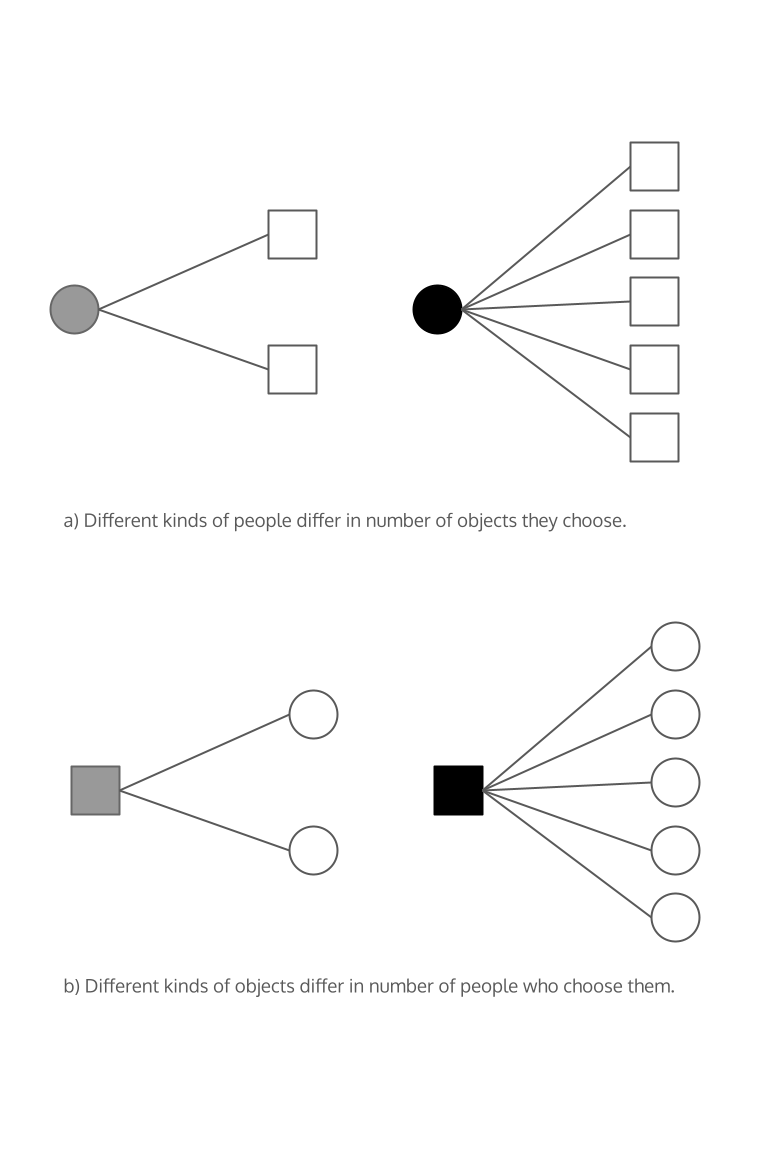
\includegraphics[width=1.0\linewidth]{Figs/local-struct1.png}
    \caption{Local structural neighborhoods of omnivorousness and populairty}
    \label{fig:local-struct1}
\end{figure}
\end{document}

\endinput
%%
%% End of file `elsarticle-template-harv.tex'.
